\section{Introduction}

Knowledge Graph (KG) has been deployed in a large amount of companies nowadays. In e-commerce scenario, KGs can benefit a lot of downstream tasks, such as Product Search Relevance (PSR), recommendation, Question Answering (QA) etc. In this paper, we focus on utilizing KG to improve PSR task in e-commerce. 

In life service scenario, huge variety of products makes PSR task more challenging. In such scenario, product category covers almost all products you can see in all markets and shops in one city, including all kinds of fruits, vegetables, snacks etc. One of the most challenging problem in such scenario is that you may not know what a product exactly is with only product name as they may have various synonyms, especially in Chinese. Apart from synonyms, typos also add difficulty to this task. All these challenges make external knowledge necessary for this task. 

% \sansa{Emphasizing Chinese narrows the scope of motivation}
% \zelin{suggestion: ... are comprehensively understood by the model}
% \zelin{the world?}
The core idea of fusing KG into PSR model is that with the help of KG, query intent and product essence can be comprehensively understood by the model, which means KG can help model understand objective things better. The overview of PSR task with KG in e-commerce is depicted in Figure \ref{fig:taskoverview}. Generally speaking, there is usually a hierarchical taxonomy to organize items and concepts in e-commerce KG. This taxonomy is usually manually defined and coarse-grained, for example, ``Vegetable / Rhizomes / Potato'' is a three-level path in taxonomy. To better understand user needs and describe essence of products, more fine-grained e-commerce related concept graph is usually constructed. For these concepts in KG, some necessary relations, such as \textit{synonym} and \textit{related\_to}, are also defined to clarify the relationship between different concepts. Generally speaking, this KG framework is adopted in AliCoCo \cite{luo2020alicoco, luo2021alicoco2}, Xiaomi product KG \cite{xiaomi} and our scenario etc., although different companies have different design for their own scenario. Specifically, in our scenario, the product taxonomy is a manually constructed tree structure connected by isA relationships. 
Apart from the taxonomy, a fine-grained e-commerce concept graph is also constructed. 

% \zelin{product taxonomy -> category taxonomy? we should say each product links to one category?}
% \zelin{``this KG framework'' is not depicted clearly enough}
% \sansa{\sout{Only alicoco? no other works?}}
% \sansa{\sout{use a different font}}

% However, current knowledge fusion methods cannot make full use of the KG and help model essentially understand textual information.

% \begin{figure*}[thbp] \centering
%     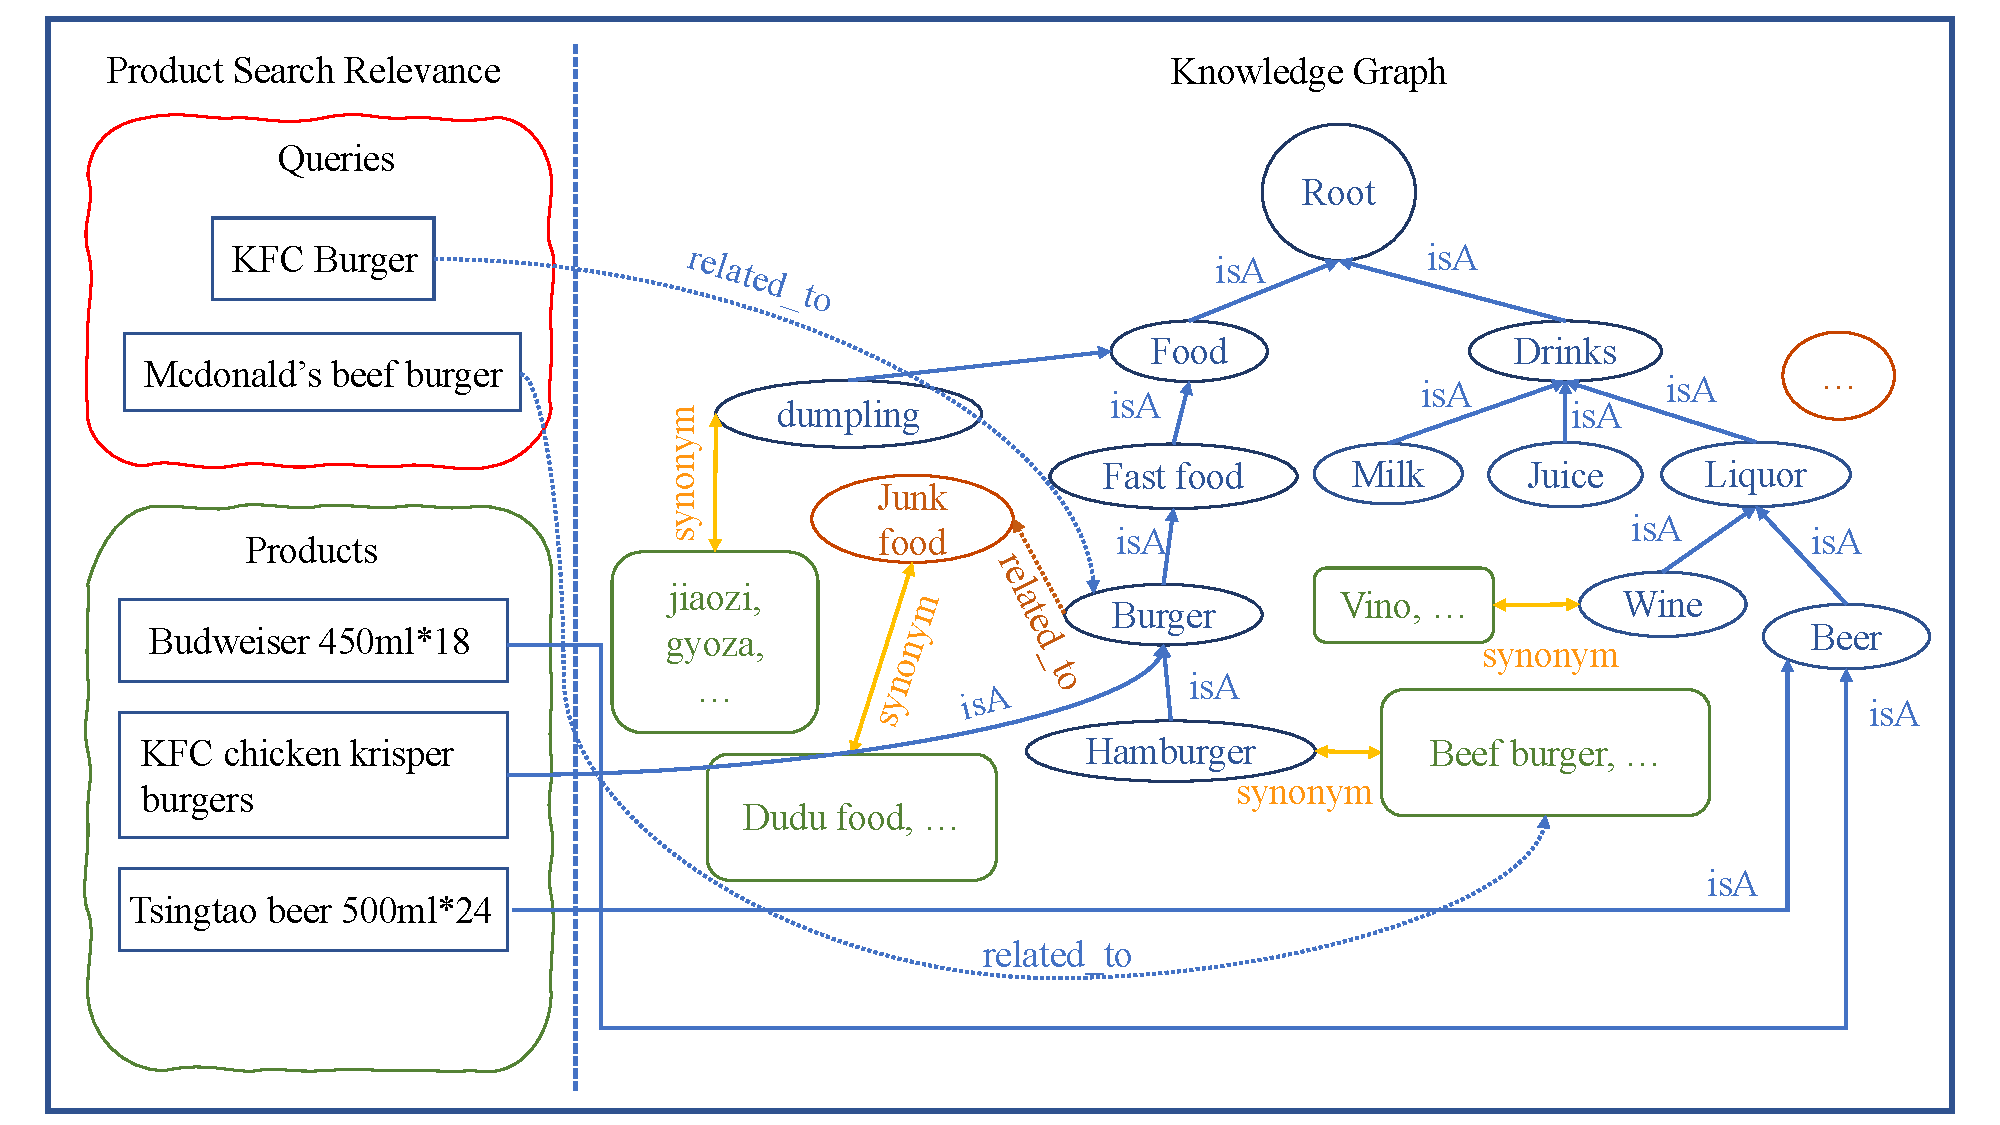
\includegraphics[width=0.99\textwidth]{task_overview_2}
%     \caption{Overview of \textit{Knowledge Graph based Product Search Relevance (KGPSR) Task}.}
%     \label{fig:taskoverview}
% \end{figure*}

\begin{figure}[th] \centering
    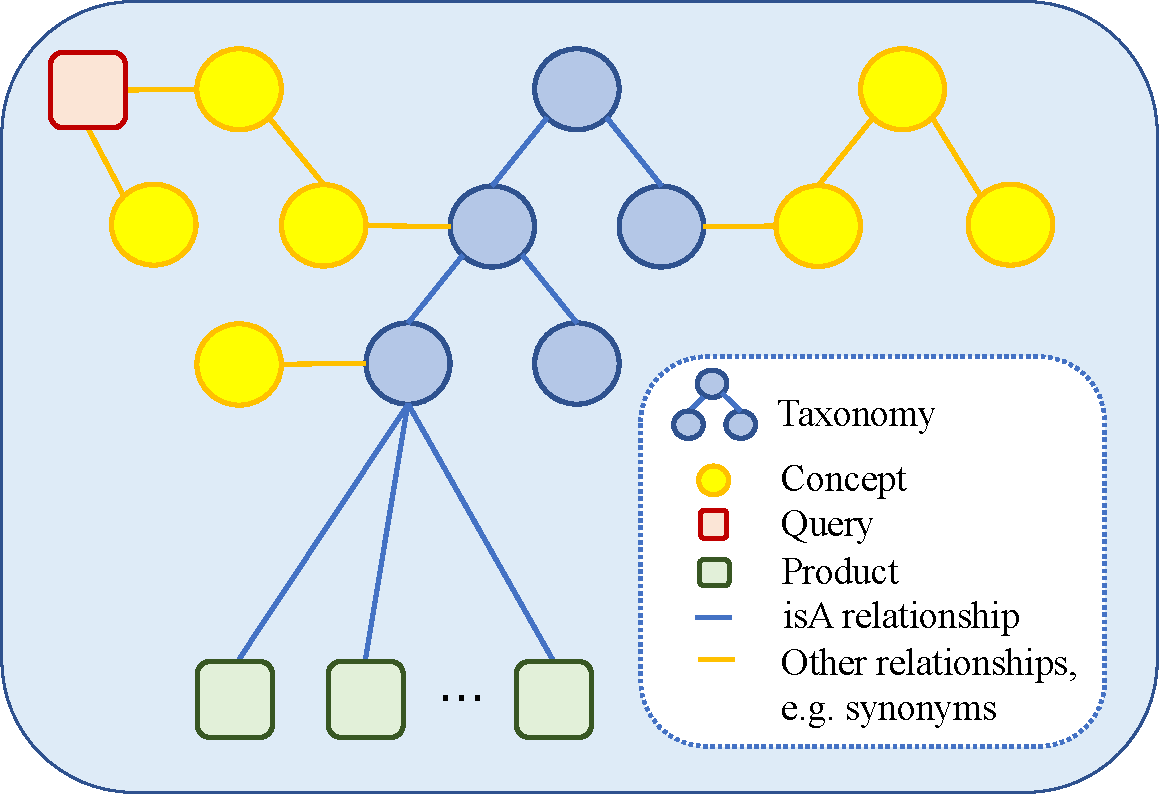
\includegraphics[width=0.4\textwidth]{task_overview3}
    \caption{Overview of Product Search Relevance task with Knowledge Graph. In such task, given a pair of query and product, a PSR model needs to measure the relevance between the query and product with the help of KG.}
    \label{fig:taskoverview}
\end{figure}

% \sansa{\sout{totally unclear about the task. I thought this figure is about the KG structure. You named it TASK, then what is the input and output?}}
% \sansa{\sout{why methods for longer text cannot.} also need citation for the whole paragraph.}

% Currently, due to the short length of both query and product, KG fusion methods can be applied are relatively limited. 

% The most common approaches to fuse KG knowledge into model, such as Knowledge Graph Path (KGP) concatenation \cite{bian2021benchmarking}, Knowledge Graph Embedding (KGE) fusion \cite{luo2021alicoco2}, etc. can only fuse knowledge in a shallow form. 


KG contains different kinds of knowledge to be mined. Lots of hidden knowledge, including hypernyms, hyponyms, synonyms, and KG structure, is waiting to be exploited. In downstream tasks, knowledge is usually utilized in a relatively straightforward and shallow way \cite{bian2021benchmarking, luo2020alicoco, luo2021alicoco2, zhang2021enriching}, such as string concatenation, and embedding fusion, etc. These knowledge fusion methods are good at fusing positive relationship knowledge to tell model what an unknown entity or concept is, but there are still problems that cannot be solved in our scenario. One limitation of these methods is that they have less ability to make use of negative relationship knowledge in KG to teach model to distinguish between two vague concepts or entities well when positive relationship knowledge is insufficient. This means relationships between concepts or entities in KG are not fused well into model. For example, for the query product pair ``Green onion'' and ``Seaweed-flavored shallots green onion 65g'' (a kind of snack), even though the positive relationship knowledge of the product in KG ``Snacks / Fried food \& puffed food / Others'', is concatenated to the product name to tell the model they are not the same thing, the similarity between the query and product is still high, which means model ignores the fused positive relationship knowledge. This kind of knowledge ignorance problem is usually caused by lexical domination, which means the semantic of product is dominated by text that appears in both query and product. In this case, ``green onion'' dominates model's understanding of this product. This problem is more significant in our scenario as query and product name are usually short.

% \zelin{sentence too long, hard to understand}
% However, knowledge in KG cannot be deeply mined and utilized by these methods. 

% \zelin{any evidence supporting this statement?}

% \zelin{we'd better explain what is `lexical domination' and cite some works encountering `lexical domination'?}

% Specifically, correct knowledge can be ignored by model with current fusion approach sometimes. 



% In our application scenario, there are still problems cannot be solved by these methods and these problems are mainly caused by \textbf{Underutilized Knowledge Challenge}. 



% However, current methods mainly focus on fuse knowledge by string or embedding concatenation and cannot help model understand the relationship between current query/product and other entities/concepts in KG fundamentally. 

% mine knowledge from KG. 

% In KG construction, products are usually linked to KG by human efforts or models, and both methods will inevitably introduce noise. For instance, product ``Beer Partner 180g/bag'' (a kind of snack) can be mis-linked on the path of ``Snacks - cakes and pastries - bread'' in KG taxonomy. Apperantly, fusing such kind of noisy knowledge in a direct manner does harm to model performance easily. Even though, sometimes knowledge is correct, fusing irrelevant knowledge directly can also cause semantic drift, and this kind of knowledge is also another form of noise. We define this challenge as \textbf{Noisy Knowledge Challenge} in this paper. 

% First, from the perspective of query side, query is usually shorter and contains less information. 

% One critical limitation of conventional knowledge fusion methods 



% This problem is defined as Knowledge Ignorance problem. \sansa{you define a challenge, and then a problem, a little bit weird}

% \sansa{\sout{You just list one problem?}}
% \zelin{... optimize the alignment and uniformity of product text embeddings}
In order to solve the problem mentioned above, negative relationship knowledge is necessary to be further utilized to tell the model what the product is not. Thus, we design a novel KG fusion method with contrastive learning called Knowledge Graph \textbf{Con}trastive  \textbf{Fu}sion (ConFu) to utilize different kinds of relationship knowledge in KG better. Our core idea is that model can learn relationships among query/product and other concepts or entities in KG through contrastive learning task to understand user intent and product essence. Specifically, with query-side contrastive learning, ConFu can learn knowledge like synonyms and hypernyms of query and learn to distinguish irrelevant queries. With product-side contrastive learning, ConFu can learn relationships among different products and have a stronger ability to distinguish ambiguous products. 
For the case we mentioned above, ConFu can solve the problem using contrastive learning by embedding ``green onion'' and the product into different regions in semantic space.
Another advantage of ConFu is that it does not need external knowledge any more during inferece stage. 

Generally speaking, our key contributions are summarized as follows: 

\begin{itemize}
    \item \textbf{A KG based PSR Dataset}. In this paper, we release a novel PSR dataset with KG in life-service scenario to call for better solutions. As far as we know, we are the first to release such a Chinese PSR data set with KG. 
    \item \textbf{A Novel KG Fusion Method}. We propose a novel fusion method to inject knowledge in KG into PSR model. With query-side contrastive fusion and product-side contrastive fusion, knowledge in KG can be effectively fused into model to help model understand user need and product essence.
    \item \textbf{Effectiveness}. According to our experiments, ConFu can successfully fuse KG into PSR model and benefits PSR task. ConFu outperforms all other baseline methods on KGPSR task by more than 2 points on AUC score. Visualization and case study also demonstrate the effectiveness of ConFu. 
\end{itemize}

% \sansa{\sout{list some specific numbers}}

% \sansa{\sout{Too much space for motivations but no space for methods. Just one sentence for methods?}}
%  With contrastive learning, both positive relationship knowledge and negative relationship knowledge can be injected into model.